% sections/comparison.tex
\section{Comparative Analysis: DRAM vs FeRAM}
\label{sec:comparison}

Table~\ref{tab:comparison} summarizes representative literature values for DRAM and FeRAM. DRAM provides high speed and very low energy/bit but requires periodic refresh due to short intrinsic retention \cite{choi2022,kim2021_dram,iedm2023_dram}. FeRAM offers non-volatility with retention beyond $10^{5}$~s and endurance reported in the $10^{12}$--$10^{13}$ range for optimized HfO$_2$ stacks, typically at higher write energy per bit \cite{boscke2011,mueller2012,noheda2023,martin2020}.

\begin{table}[!t]
\centering
\caption{Representative metrics (order-of-magnitude, literature indications).}
\label{tab:comparison}
\begin{tabular}{lcccc}
\toprule
Tech. & Speed (ns) & Retention (s) & Endurance & Energy/bit \\
\midrule
DRAM  & $\le 10$  & $\sim 10^{-2}$ to $10^{-1}$ & $\ge 10^{16}$ & $10$--$100$ fJ \\
FeRAM & $\le 50$  & $\ge 10^{5}$                & $10^{12}$--$10^{13}$ & $10^{2}$--$10^{3}$ fJ \\
\bottomrule
\end{tabular}
\end{table}

Figures~\ref{fig:speed_retention} and \ref{fig:energy_speed} conceptually illustrate the speed--retention and energy--speed trade-offs, respectively.

% --- Fig.1: Speed vs. retention (log-log) ---
\begin{figure}[!t]
  \centering
  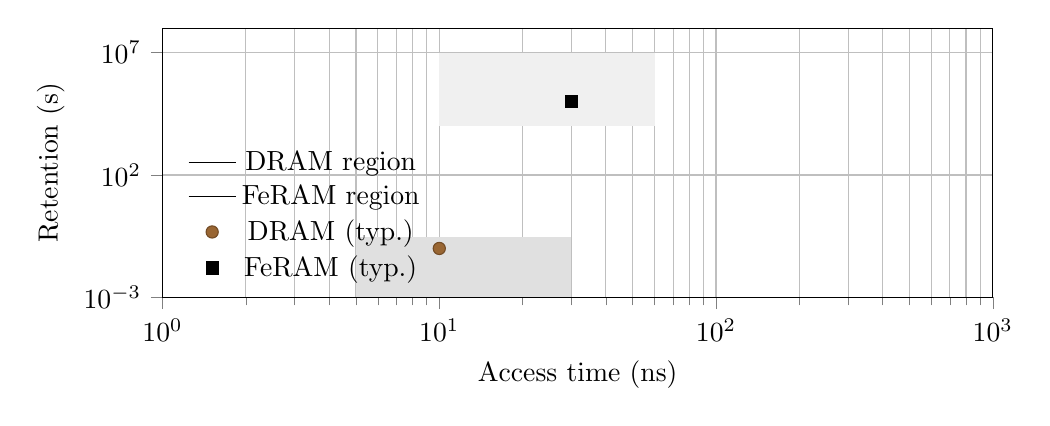
\begin{tikzpicture}
    \begin{loglogaxis}[
      width=\linewidth,
      height=5.0cm,
      xlabel={Access time (ns)},
      ylabel={Retention (s)},
      xmin=1e0, xmax=1e3,
      ymin=1e-3, ymax=1e8,
      legend style={at={(0.02,0.02)},anchor=south west,draw=none,fill=none},
      tick align=outside,
      tick pos=left,
      grid=both,
    ]
      % DRAM operating region (rough)
      \addplot[draw=none, fill=black!12] coordinates {
        (5,1e-3) (30,1e-3) (30,3e-1) (5,3e-1)
      } -- cycle;
      % FeRAM operating region (rough)
      \addplot[draw=none, fill=black!6] coordinates {
        (10,1e4) (60,1e4) (60,1e7) (10,1e7)
      } -- cycle;

      % Representative points
      \addplot+[only marks, mark=*, mark size=2.2pt] coordinates {(10,1e-1)}; % DRAM
      \addplot+[only marks, mark=square*, mark size=2.2pt] coordinates {(30,1e5)}; % FeRAM

      \legend{DRAM region, FeRAM region, DRAM (typ.), FeRAM (typ.)}
    \end{loglogaxis}
  \end{tikzpicture}
  \caption{Conceptual trade-off between access time and retention. DRAM is faster but requires refresh (short retention), whereas FeRAM provides long retention at modest access times.}
  \label{fig:speed_retention}
\end{figure}

% --- Fig.2: Write energy per bit vs. write speed (log-log) ---
\begin{figure}[!t]
  \centering
  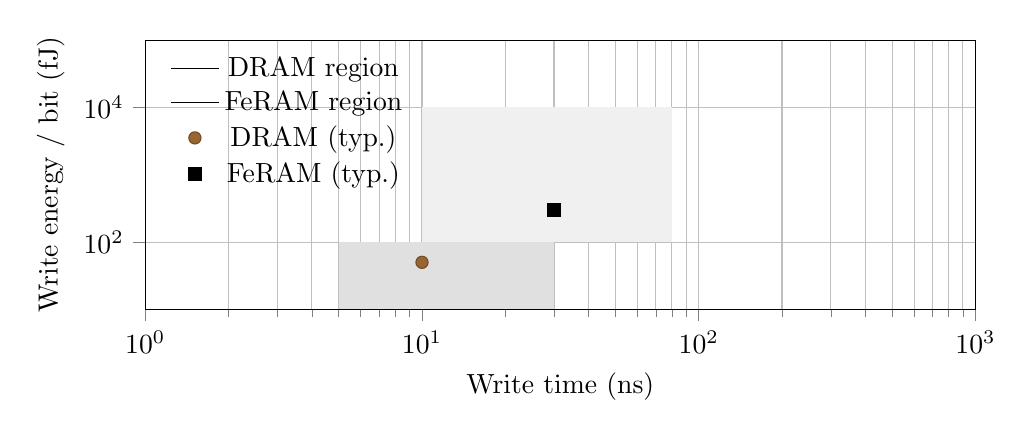
\begin{tikzpicture}
    \begin{loglogaxis}[
      width=\linewidth,
      height=5.0cm,
      xlabel={Write time (ns)},
      ylabel={Write energy / bit (fJ)},
      xmin=1e0, xmax=1e3,
      ymin=1e1, ymax=1e5,
      legend style={at={(0.02,0.98)},anchor=north west,draw=none,fill=none},
      tick align=outside,
      tick pos=left,
      grid=both,
    ]
      % DRAM energy-speed region (rough)
      \addplot[draw=none, fill=black!12] coordinates {
        (5,1e1) (30,1e1) (30,1e2) (5,1e2)
      } -- cycle;
      % FeRAM energy-speed region (rough)
      \addplot[draw=none, fill=black!6] coordinates {
        (10,1e2) (80,1e2) (80,1e4) (10,1e4)
      } -- cycle;

      % Representative points
      \addplot+[only marks, mark=*, mark size=2.2pt] coordinates {(10,5e1)};   % DRAM
      \addplot+[only marks, mark=square*, mark size=2.2pt] coordinates {(30,3e2)}; % FeRAM

      \legend{DRAM region, FeRAM region, DRAM (typ.), FeRAM (typ.)}
    \end{loglogaxis}
  \end{tikzpicture}
  \caption{Conceptual write energy versus write time. DRAM typically achieves lower energy/bit at short write times; FeRAM writes cost more energy but persist without refresh.}
  \label{fig:energy_speed}
\end{figure}
